\section{Parser Vertiefung}
\subsection{Abstrakter Syntaxbaum Design}
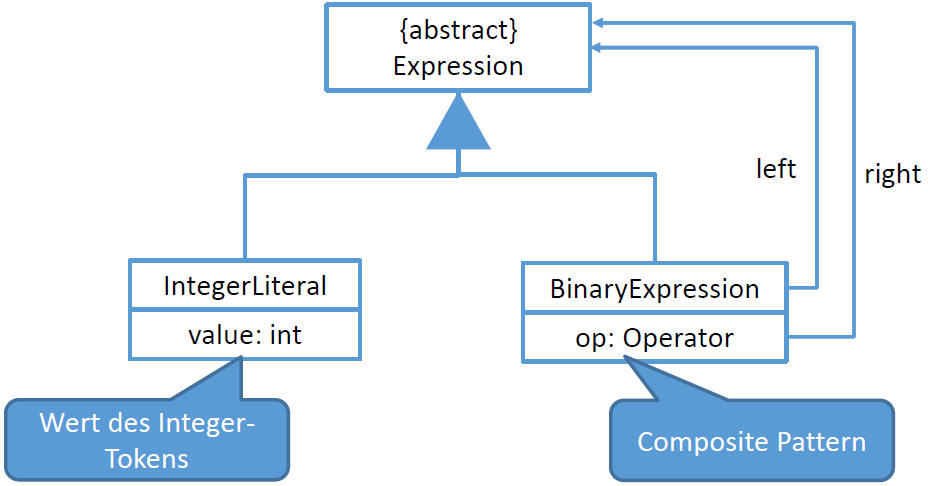
\includegraphics[width=0.7\linewidth]{syntaxbaum_design.png}

\subsection{Bottom-Up Parsing}
\begin{itemize}
    \item Mächtiger als LL (Top-Down) Parser
    \item Kann Linksrekursion behandeln
\end{itemize}
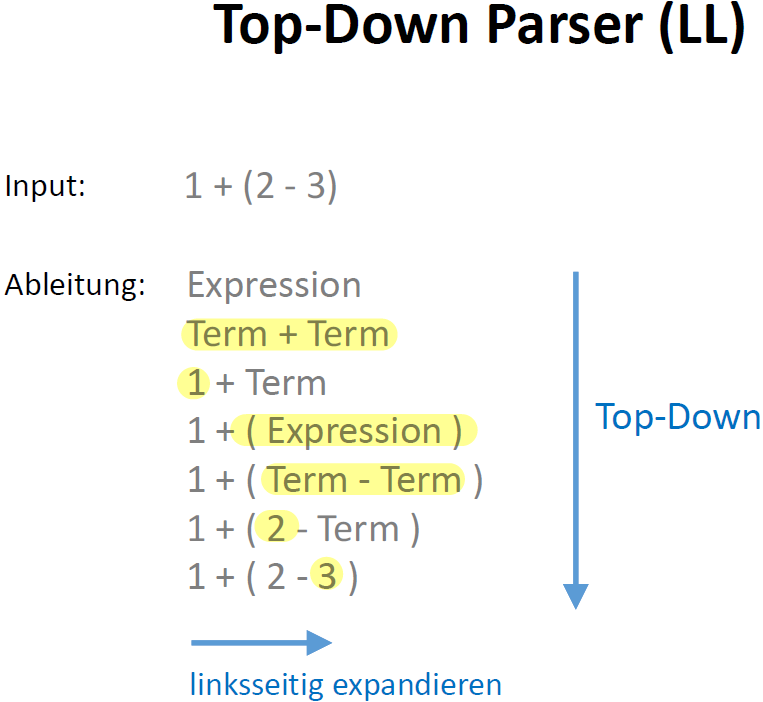
\includegraphics[width=0.5\linewidth]{top_down2.png}
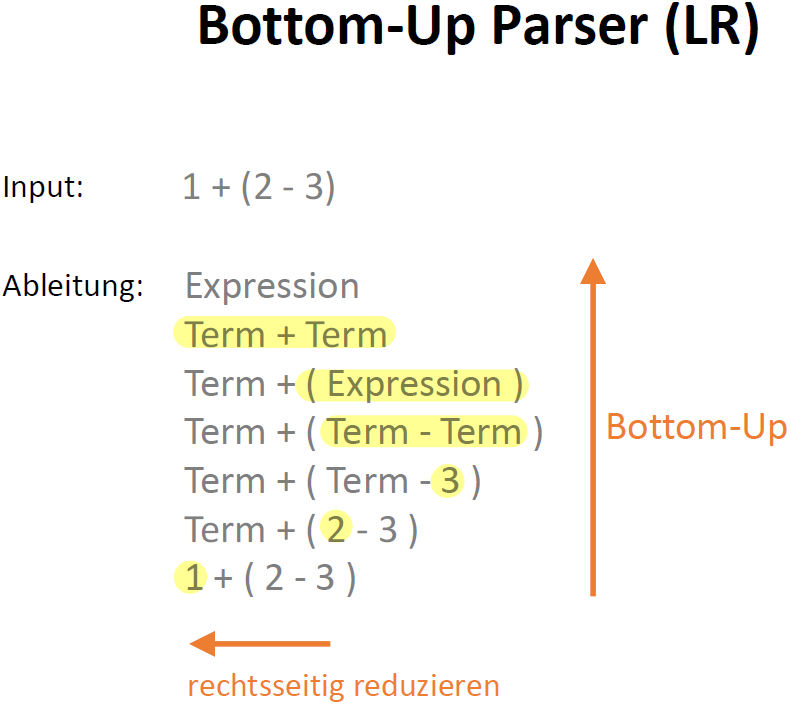
\includegraphics[width=0.5\linewidth]{bottom_up2.png}

\subsubsection{Ansatz}
\begin{itemize}
    \item Lese Symbole im Text ohne fixes Ziel
    \item Prüfe nach jedem Schritt, ob gelesene Folge Produktion entspricht
    \begin{itemize}
        \item Wenn ja: Reduziere auf Syntaxkonstrukt (REDUCE)
        \item Wenn nein: Lese weiteres Symbol im Text (SHIFT)
    \end{itemize}
    \item Am Schluss bleibt Startsymbol übrig, sonst Syntaxfehler
\end{itemize}

\subsubsection{Beispielablauf}
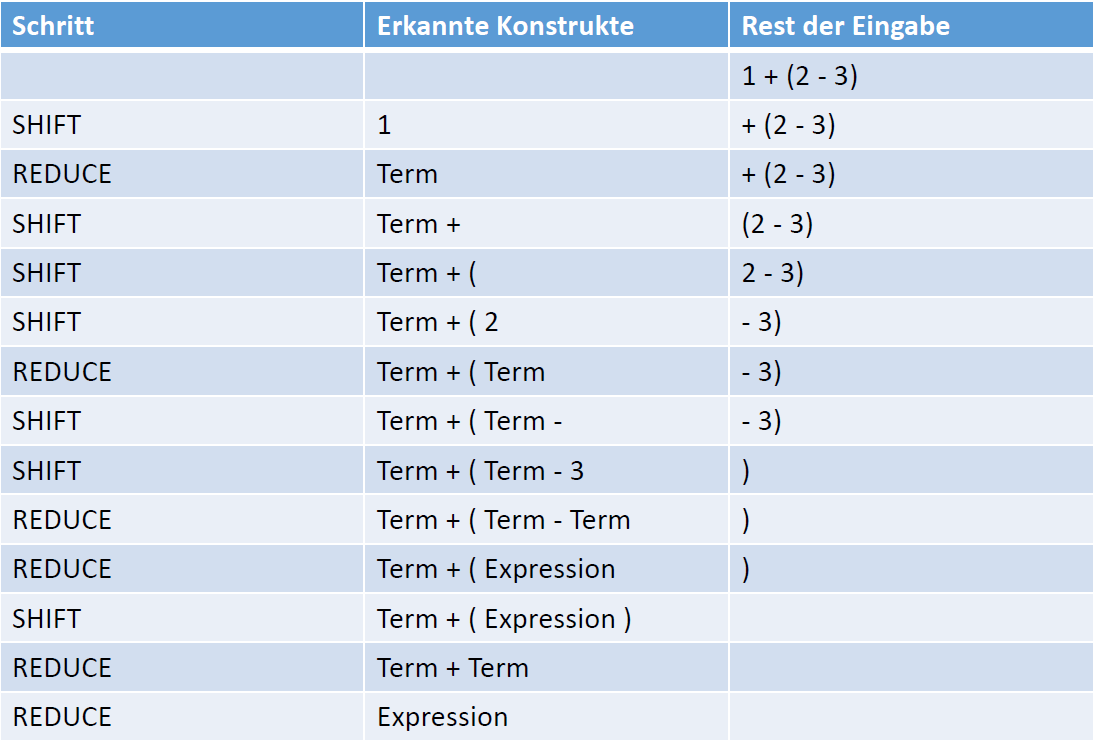
\includegraphics[width=0.7\linewidth]{bottom_up_ablauf.png}
\subsubsection{Parser Tabelle - Vereinfacht}
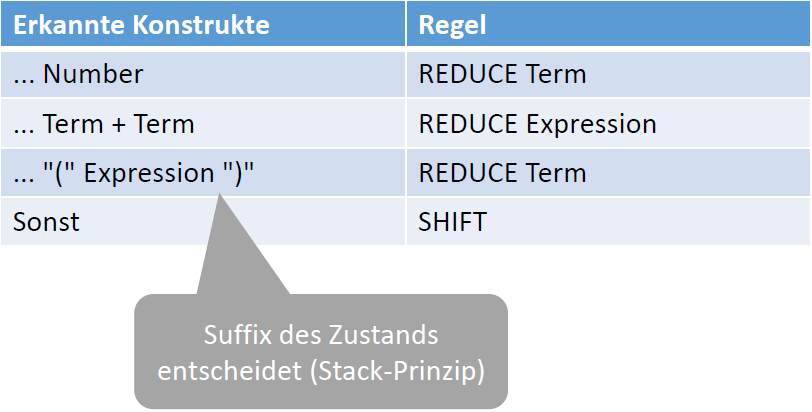
\includegraphics[width=0.5\linewidth]{parser_tabelle_vereinfacht.png}

\subsection{LR-Parser (Bottom-Up) Varianten}
\textbf{LR(0)}
\begin{itemize}
    \item Parse Tabelle ohne Lookahead erstellen
    \item Zustand reicht, um zu entscheiden
\end{itemize}
\textbf{SLR(k) (Simple LR)}
\begin{itemize}
    \item Lookahead bei REDUCE, um Konflikt zu lösen
    \item Keine neuen Zustände
\end{itemize}
\textbf{LALR(k) (Look-Ahead LR)}
\begin{itemize}
    \item Analysiert Sprache auf LR(0)-Konflikte
    \item Benutzt Lookahead bei Konfliktstellen mit neuen Zuständen
\end{itemize}
\textbf{LR(k)}
\begin{itemize}
    \item Pro Grammatikschritt + Lookahead ein Zustand
    \item Nicht praxistauglich, zu viele Zustände
\end{itemize}